COORDINATES
6.87168 7.65929 8.15501

\section{Data}
\begin{itemize}
	\item 10 sensors
	\item $T_{transmission} = 10 \text{ minutes}$
	\item $b = 2000 \text{ bit}$
	\item $E_b = 5 \text{ mJ}$
	\item $E_c = 50 \text{ nJ/bit}$
	\item $E_{tx} = k \cdot d^2 \text{ nJ/bit}$
	\item $k = 1 \text{ nJ/bit/$m^2$}$
\end{itemize}
\begin{table}[H]
\centering 
\begin{tabular}{| c | c |}
	\hline 
	\rowcolor{bluepoli!40}
	\textbf{Sensor} & \textbf{Position}\T\B \\
	\hline 
	1 & (1, 2) \T\B\\
	2 &(10, 3) \T\B\\
	3 & (4, 8) \T\B\\
	4 & (15, 7) \T\B\\
	5  & (6, 1) \T\B\\
	6  & (9, 12) \T\B\\
	7  & (14, 4) \T\B\\
	8  & (3, 10) \T\B\\
	9  & (7, 7) \T\B\\
	10  & (12, 14) \T\B\\
	\hline
\end{tabular}
\\[10pt]
\caption{Sensor position table}
\label{table:sensor_position_table}
\end{table}

\begin{figure}[H]
    \centering
    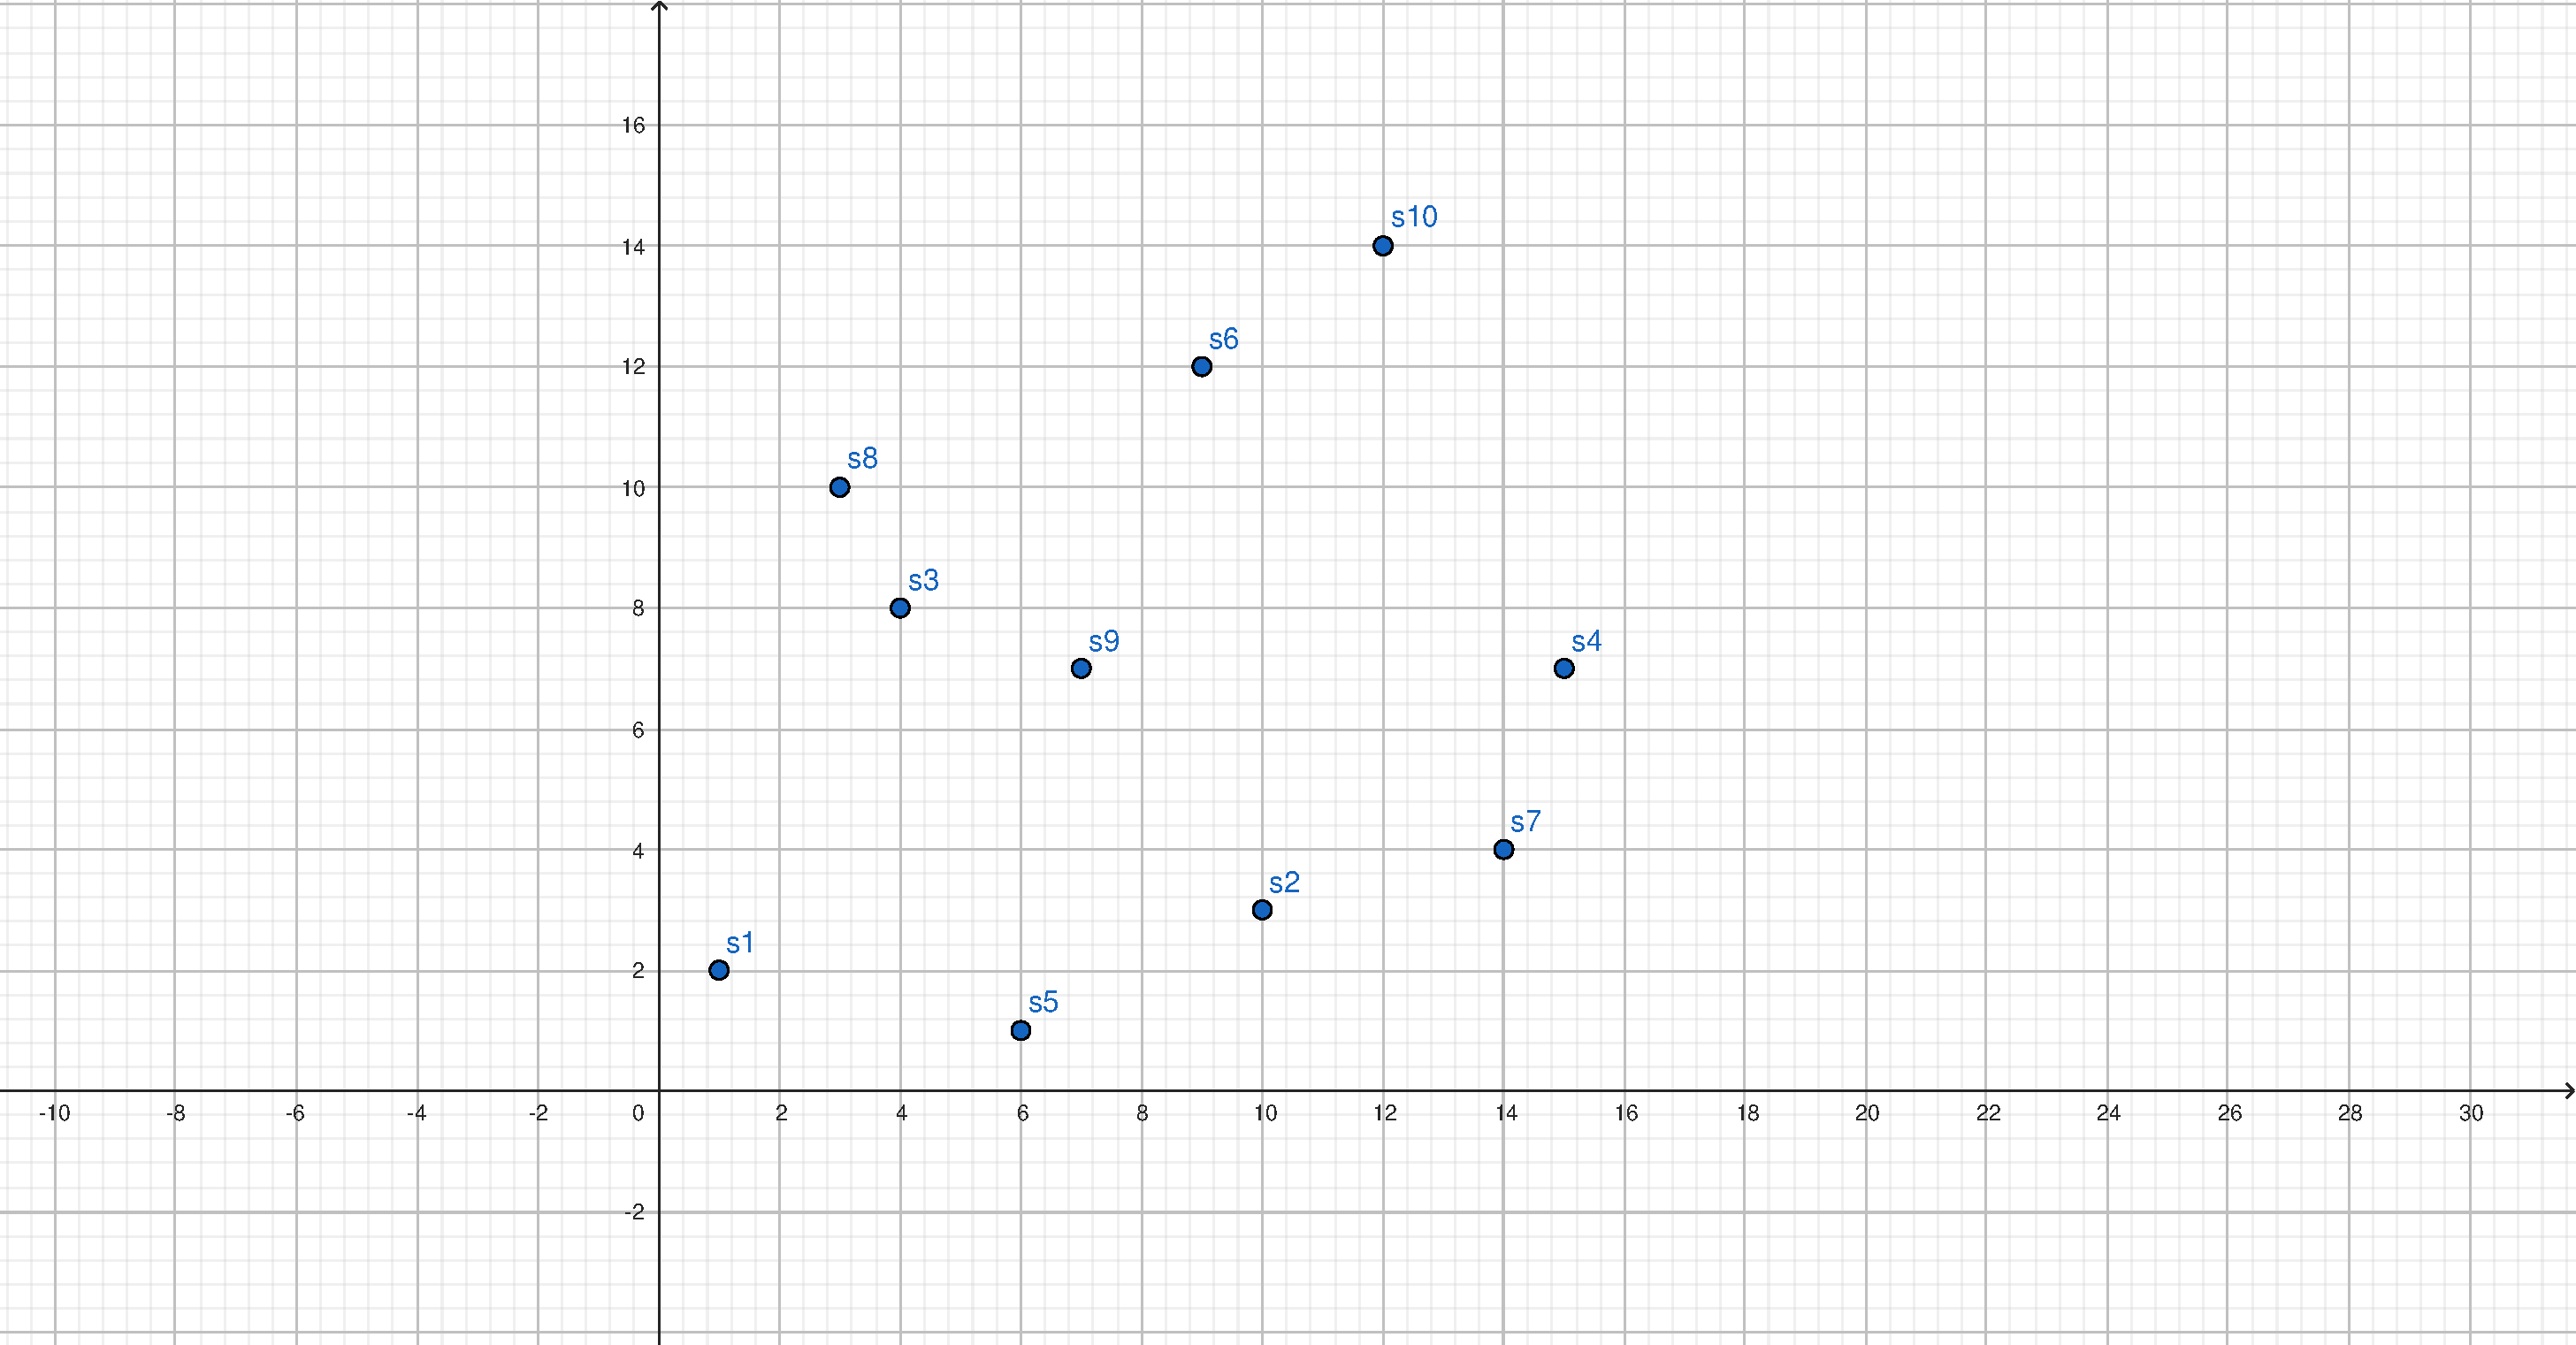
\includegraphics[width=\linewidth, height=0.4\textheight, keepaspectratio]{points.pdf.pdf}
    \caption{Sensor distribution}
    \label{fig:Sensor_distribution}
\end{figure}

\section{Point A}
Sink position = ($x_s, y_s$) = (20, 20)\\


We calculated the distance of the farer sensor (sensor 1) from the sink using the cartesian distance: \[ distance_1 = d \{(1, 2) , (20, 20)\} = \sqrt{(20-1)^2 + (20-2)^2} = \sqrt{685} m \]

\[
E_{cycle, 1} = E_c \cdot b + E_{tx(1)} = 50 nJ/bit \cdot 2000 \text{ bit} + 1 nJ/bit/m^2 \cdot 685 m^2 \cdot 2000 \text{ bit} = 1.47 \cdot 10^{-3} J
\]

\[
n = \text{# cycles} = E_b / E_{cycle, 1} = 3.4 cycles
\]
Assuming that each sensor transmits at the beginning of the ten minutes, the system will last for 3 cycles and during the fourth cycle the farer sensor will die.

\section{Point B}









